% Options for packages loaded elsewhere
\PassOptionsToPackage{unicode}{hyperref}
\PassOptionsToPackage{hyphens}{url}
%
\documentclass[
]{book}
\usepackage{lmodern}
\usepackage{amssymb,amsmath}
\usepackage{ifxetex,ifluatex}
\ifnum 0\ifxetex 1\fi\ifluatex 1\fi=0 % if pdftex
  \usepackage[T1]{fontenc}
  \usepackage[utf8]{inputenc}
  \usepackage{textcomp} % provide euro and other symbols
\else % if luatex or xetex
  \usepackage{unicode-math}
  \defaultfontfeatures{Scale=MatchLowercase}
  \defaultfontfeatures[\rmfamily]{Ligatures=TeX,Scale=1}
\fi
% Use upquote if available, for straight quotes in verbatim environments
\IfFileExists{upquote.sty}{\usepackage{upquote}}{}
\IfFileExists{microtype.sty}{% use microtype if available
  \usepackage[]{microtype}
  \UseMicrotypeSet[protrusion]{basicmath} % disable protrusion for tt fonts
}{}
\makeatletter
\@ifundefined{KOMAClassName}{% if non-KOMA class
  \IfFileExists{parskip.sty}{%
    \usepackage{parskip}
  }{% else
    \setlength{\parindent}{0pt}
    \setlength{\parskip}{6pt plus 2pt minus 1pt}}
}{% if KOMA class
  \KOMAoptions{parskip=half}}
\makeatother
\usepackage{xcolor}
\IfFileExists{xurl.sty}{\usepackage{xurl}}{} % add URL line breaks if available
\IfFileExists{bookmark.sty}{\usepackage{bookmark}}{\usepackage{hyperref}}
\hypersetup{
  pdftitle={Shiny App Workflows},
  pdfauthor={Braeden Klaver},
  hidelinks,
  pdfcreator={LaTeX via pandoc}}
\urlstyle{same} % disable monospaced font for URLs
\usepackage{color}
\usepackage{fancyvrb}
\newcommand{\VerbBar}{|}
\newcommand{\VERB}{\Verb[commandchars=\\\{\}]}
\DefineVerbatimEnvironment{Highlighting}{Verbatim}{commandchars=\\\{\}}
% Add ',fontsize=\small' for more characters per line
\usepackage{framed}
\definecolor{shadecolor}{RGB}{248,248,248}
\newenvironment{Shaded}{\begin{snugshade}}{\end{snugshade}}
\newcommand{\AlertTok}[1]{\textcolor[rgb]{0.94,0.16,0.16}{#1}}
\newcommand{\AnnotationTok}[1]{\textcolor[rgb]{0.56,0.35,0.01}{\textbf{\textit{#1}}}}
\newcommand{\AttributeTok}[1]{\textcolor[rgb]{0.77,0.63,0.00}{#1}}
\newcommand{\BaseNTok}[1]{\textcolor[rgb]{0.00,0.00,0.81}{#1}}
\newcommand{\BuiltInTok}[1]{#1}
\newcommand{\CharTok}[1]{\textcolor[rgb]{0.31,0.60,0.02}{#1}}
\newcommand{\CommentTok}[1]{\textcolor[rgb]{0.56,0.35,0.01}{\textit{#1}}}
\newcommand{\CommentVarTok}[1]{\textcolor[rgb]{0.56,0.35,0.01}{\textbf{\textit{#1}}}}
\newcommand{\ConstantTok}[1]{\textcolor[rgb]{0.00,0.00,0.00}{#1}}
\newcommand{\ControlFlowTok}[1]{\textcolor[rgb]{0.13,0.29,0.53}{\textbf{#1}}}
\newcommand{\DataTypeTok}[1]{\textcolor[rgb]{0.13,0.29,0.53}{#1}}
\newcommand{\DecValTok}[1]{\textcolor[rgb]{0.00,0.00,0.81}{#1}}
\newcommand{\DocumentationTok}[1]{\textcolor[rgb]{0.56,0.35,0.01}{\textbf{\textit{#1}}}}
\newcommand{\ErrorTok}[1]{\textcolor[rgb]{0.64,0.00,0.00}{\textbf{#1}}}
\newcommand{\ExtensionTok}[1]{#1}
\newcommand{\FloatTok}[1]{\textcolor[rgb]{0.00,0.00,0.81}{#1}}
\newcommand{\FunctionTok}[1]{\textcolor[rgb]{0.00,0.00,0.00}{#1}}
\newcommand{\ImportTok}[1]{#1}
\newcommand{\InformationTok}[1]{\textcolor[rgb]{0.56,0.35,0.01}{\textbf{\textit{#1}}}}
\newcommand{\KeywordTok}[1]{\textcolor[rgb]{0.13,0.29,0.53}{\textbf{#1}}}
\newcommand{\NormalTok}[1]{#1}
\newcommand{\OperatorTok}[1]{\textcolor[rgb]{0.81,0.36,0.00}{\textbf{#1}}}
\newcommand{\OtherTok}[1]{\textcolor[rgb]{0.56,0.35,0.01}{#1}}
\newcommand{\PreprocessorTok}[1]{\textcolor[rgb]{0.56,0.35,0.01}{\textit{#1}}}
\newcommand{\RegionMarkerTok}[1]{#1}
\newcommand{\SpecialCharTok}[1]{\textcolor[rgb]{0.00,0.00,0.00}{#1}}
\newcommand{\SpecialStringTok}[1]{\textcolor[rgb]{0.31,0.60,0.02}{#1}}
\newcommand{\StringTok}[1]{\textcolor[rgb]{0.31,0.60,0.02}{#1}}
\newcommand{\VariableTok}[1]{\textcolor[rgb]{0.00,0.00,0.00}{#1}}
\newcommand{\VerbatimStringTok}[1]{\textcolor[rgb]{0.31,0.60,0.02}{#1}}
\newcommand{\WarningTok}[1]{\textcolor[rgb]{0.56,0.35,0.01}{\textbf{\textit{#1}}}}
\usepackage{longtable,booktabs}
% Correct order of tables after \paragraph or \subparagraph
\usepackage{etoolbox}
\makeatletter
\patchcmd\longtable{\par}{\if@noskipsec\mbox{}\fi\par}{}{}
\makeatother
% Allow footnotes in longtable head/foot
\IfFileExists{footnotehyper.sty}{\usepackage{footnotehyper}}{\usepackage{footnote}}
\makesavenoteenv{longtable}
\usepackage{graphicx,grffile}
\makeatletter
\def\maxwidth{\ifdim\Gin@nat@width>\linewidth\linewidth\else\Gin@nat@width\fi}
\def\maxheight{\ifdim\Gin@nat@height>\textheight\textheight\else\Gin@nat@height\fi}
\makeatother
% Scale images if necessary, so that they will not overflow the page
% margins by default, and it is still possible to overwrite the defaults
% using explicit options in \includegraphics[width, height, ...]{}
\setkeys{Gin}{width=\maxwidth,height=\maxheight,keepaspectratio}
% Set default figure placement to htbp
\makeatletter
\def\fps@figure{htbp}
\makeatother
\setlength{\emergencystretch}{3em} % prevent overfull lines
\providecommand{\tightlist}{%
  \setlength{\itemsep}{0pt}\setlength{\parskip}{0pt}}
\setcounter{secnumdepth}{5}
\usepackage{booktabs}
\usepackage{booktabs}
\usepackage{longtable}
\usepackage{array}
\usepackage{multirow}
\usepackage{wrapfig}
\usepackage{float}
\usepackage{colortbl}
\usepackage{pdflscape}
\usepackage{tabu}
\usepackage{threeparttable}
\usepackage{threeparttablex}
\usepackage[normalem]{ulem}
\usepackage{makecell}
\usepackage{xcolor}
\usepackage[]{natbib}
\bibliographystyle{plainnat}

\title{Shiny App Workflows}
\author{Braeden Klaver}
\date{2025-03-12}

\begin{document}
\maketitle

{
\setcounter{tocdepth}{1}
\tableofcontents
}
\hypertarget{preface}{%
\chapter*{Preface}\label{preface}}
\addcontentsline{toc}{chapter}{Preface}

This document aims to provide a walkthrough on how to work within
a shiny app workflow that leverages git/gitlab, package structure,
shiny, and bslib.

\hypertarget{git}{%
\chapter{Git}\label{git}}

\href{https://git-scm.com/}{Git} is a free and open-source version control system. When used regularly and as intended, developers will have a full history of their project within a local repository. In addition to a historical log of changes to project files, git allows for project branching to support users to test/develop new code, while maintaining the master version for easy reversion. When users are ready to implement their new branch into the main codebase git can be used for merging files, whereby it tracks changes and ensures there are no conflicts between the main version and the new version.

Beyond local usage, git is also supported by web-based repositories such as \href{https://github.com/}{Github} and \href{https://about.gitlab.com/}{Gitlab}, where projects can be pushed, pulled, and cloned. These sites allow for easy collaboration with other developers and provide a number of user-friendly features that make working with git easier.

\textbf{NOTE}

In RStudio, git is accessed in the terminal or in the top right under the Git tab when Git has been initialized for the project.

\hypertarget{basic-workflow}{%
\section{Basic git workflow}\label{basic-workflow}}

Step 1) Create a project.

Step 2) Initialize git.\\
\texttt{git\ init}

Step 3) Check your project file status
\texttt{git\ status}

Step 4) Add a file to the local repo\\
\texttt{git\ add\ filename.R}

Step 5) Commit your change with a message\\
\texttt{git\ commit\ -m\ "Add\ filename.R"}

Step 6) Create a branch to test/develop code\\
\texttt{git\ branch\ test\_branch}

Step 7) Go into that branch\\
\texttt{git\ checkout\ test\_branch}

Step 8) Modify your code and repeat steps 3 and 4

Step 9) When ready merge branches\\
\texttt{git\ merge\ master\ test\_branch}

\textbf{TIP}

Branching is useful when you have a stable codebase that you do not want to break or if you are working collaboratively on a code base. You can create a branch to do development work and test new features until it's ready for integration with the stable codebase or your coworkers. If you are developing something from scratch by yourself you may not need to use branching until later.

\hypertarget{setting-up-github-or-gitlab-projects}{%
\section{Setting up Github or Gitlab projects}\label{setting-up-github-or-gitlab-projects}}

Ensure your profile is set up\\
\texttt{git\ config\ -\/-global\ user.name\ "Braeden\ Klaver"}~\\
\texttt{git\ config\ -\/-global\ user.email\ "braeden.klaver@bccdc.ca"}

\hypertarget{pre-existing-project-on-github-or-gitlab}{%
\subsection{Pre-existing project on Github or Gitlab}\label{pre-existing-project-on-github-or-gitlab}}

Step 1) In your terminal navigate to the folder you want to clone the project to\\
\texttt{cd\ "U:/myprojects"}

Step 2) Clone the project into that folder and give the project a name\\
\texttt{git\ clone\ http://lvmgenodh01.phsabc.ehcnet.ca/braeden.klaver/test.git\ myproject}

\hypertarget{personal-project-without-git}{%
\subsection{Personal project without git}\label{personal-project-without-git}}

Step 1) Open your R project

Step 2) Initialize git\\
\texttt{git\ init}

Step 3) Create a project on \href{https://about.gitlab.com/}{Gitlab} or \href{https://github.com/}{Github}

Step 4) Connect your R project to that repository (should be the URL)\\
\texttt{git\ remote\ add\ origin\ http://lvmgenodh01.phsabc.ehcnet.ca/braeden.klaver/test.git}

Step 5) Add and commit your files\\
\texttt{git\ add\ .}~\\
\texttt{git\ commit\ -m\ "Initial\ commit"}

Step 6) Push your project to that repository\\
\texttt{git\ push}

\hypertarget{personal-project-with-git}{%
\subsection{Personal project with Git}\label{personal-project-with-git}}

Step 1) Open your R project

Step 2) Connect your R project to that repository (should be the URL)\\
\texttt{git\ remote\ add\ origin\ http://lvmgenodh01.phsabc.ehcnet.ca/braeden.klaver/test.git}

Step 3) Push your project to that repository\\
\texttt{git\ push}

\hypertarget{collaborative-git-workflow}{%
\section{Collaborative git workflow}\label{collaborative-git-workflow}}

In addition to the basic workflow, when working with a web-based repository like \href{https://github.com/}{Github} or \href{https://about.gitlab.com/}{Gitlab} there are additional steps you will need to take:

Step 1) Pulling changes from the repository - your coworkers may have made changes!\\
\texttt{git\ pull}

Step 2) Follow the basic workflow (Section \ref{basic-workflow})

Step 3) Pushing your changes to the repository - your coworkers will want to be up to date!\\
\texttt{git\ push}

\hypertarget{using-git-at-the-bccdc}{%
\section{Using Git at the BCCDC}\label{using-git-at-the-bccdc}}

\hypertarget{git-on-citrix}{%
\subsection{Git on Citrix}\label{git-on-citrix}}

\href{https://git-scm.com/}{Git} is installed on citrix already, it can be initialized as described above or you can click a check box to create a git repository when creating a new project.

\textbf{TIP}

If you have a local R installation and you'd like to work there but do not have git installed locally you can still leverage citrix R to use git for your projects.

\hypertarget{github}{%
\subsection{Github}\label{github}}

Because \href{https://github.com/}{Github} is an external web-based repository there are some considerations for its use at the BCCDC. Currently, there are no formal guidelines on using it, for this reason using it for BCCDC-specific projects should be avoided.

\hypertarget{gitlab}{%
\subsection{Gitlab}\label{gitlab}}

The BCCDC has a private \href{http://lvmgenodh01.phsabc.ehcnet.ca/}{Gitlab repository}, which can be used for regular BCCDC projects within the scope set out in the \href{https://healthbc-my.sharepoint.com/:w:/r/personal/kathleen_mclean_bccdc_ca/Documents/GitLab\%20Guideline\%20for\%20distribution.docx?d=w2584389db5be4a7d8dc59ed28080e351\&csf=1\&web=1\&e=OH30gE}{guiding document}.

\textbf{NOTE}

You can request access to Gitlab via this \href{https://surveys.vch.ca/Survey.aspx?s=62de2ddc1daf413091a8e063d80428cd}{form}.

\hypertarget{suggested-project-workflow}{%
\subsection{Suggested project workflow}\label{suggested-project-workflow}}

Working with git tracked projects requires you to have your own local repository. For this reason, it is recommended to keep this repository in your \texttt{U:/} drive. In addition, we would recommend having another local repository in the \texttt{O:/} drive, which would be dedicated to running pipelines or deploying apps and \textbf{not} for development work.

\textbf{WARNING}

Some project data may not be permitted on your \texttt{U:/} drive, therefore ensure your code is loading that data from an appropriate location.

\hypertarget{basic-git-commands-summary}{%
\section{Basic Git Commands Summary}\label{basic-git-commands-summary}}

\begin{tabular}{l|l}
\hline
Command & Description\\
\hline
git init & Initialize git for the directory\\
\hline
git status & Check the status of files in the directory (eg. are they being tracked, have they been modified)\\
\hline
git add & Stage a file for commit\\
\hline
git rm & Remove a file staged for commit\\
\hline
git commit & Commit your changes\\
\hline
git branch & Create a branch for development work\\
\hline
git checkout & Checkout a branch to work within\\
\hline
git merge & Merge two branches together\\
\hline
git pull & Pull the most up-to-date repository from a remote (ie. Github or Gitlab)\\
\hline
git push & Push your changes to a remote repository (ie. Github or Gitlab)\\
\hline
\end{tabular}

\textbf{NOTE}

There are many other functions that you can use in git beyond those listed above, however, these give you the tools to get started.

\hypertarget{additional-resources}{%
\section{Additional Resources}\label{additional-resources}}

\begin{itemize}
\tightlist
\item
  \href{https://healthbc-my.sharepoint.com/personal/michael_kuo_bccdc_ca/_layouts/15/onedrive.aspx?id=\%2Fpersonal\%2Fmichael\%5Fkuo\%5Fbccdc\%5Fca\%2FDocuments\%2FMicrosoft\%20Teams\%20Chat\%20Files\%2Fversion\%5Fcontrol\%5Ftutorial\%2Ehtml\&parent=\%2Fpersonal\%2Fmichael\%5Fkuo\%5Fbccdc\%5Fca\%2FDocuments\%2FMicrosoft\%20Teams\%20Chat\%20Files\&ga=1}{Mike Kuo's Git Tutorial}\\
\item
  \href{https://learngitbranching.js.org/}{Git Playground}
\end{itemize}

\hypertarget{package-development}{%
\chapter{Package Development}\label{package-development}}

In R, the fundamental unit of shareable code is the package. A package bundles together code, data, documentation, and tests, and is easy to share with others.

But packages are useful even if you never share your code. As Hilary Parker says in her introduction to packages: ``Seriously, it doesn't have to be about sharing your code (although that is an added benefit!). It is about saving yourself time.'' Organising code in a package makes your life easier because packages come with conventions. For example, you put R code in \texttt{R/}, you put tests in \texttt{tests/} and you put data in \texttt{data/}. These conventions are helpful because:

\begin{itemize}
\item
  They save time --- you don't need to think about the best way to organise a project, you can just follow a template.
\item
  Standardised conventions lead to standardised tools --- if you buy into R's package conventions, you get many tools for free.
\end{itemize}

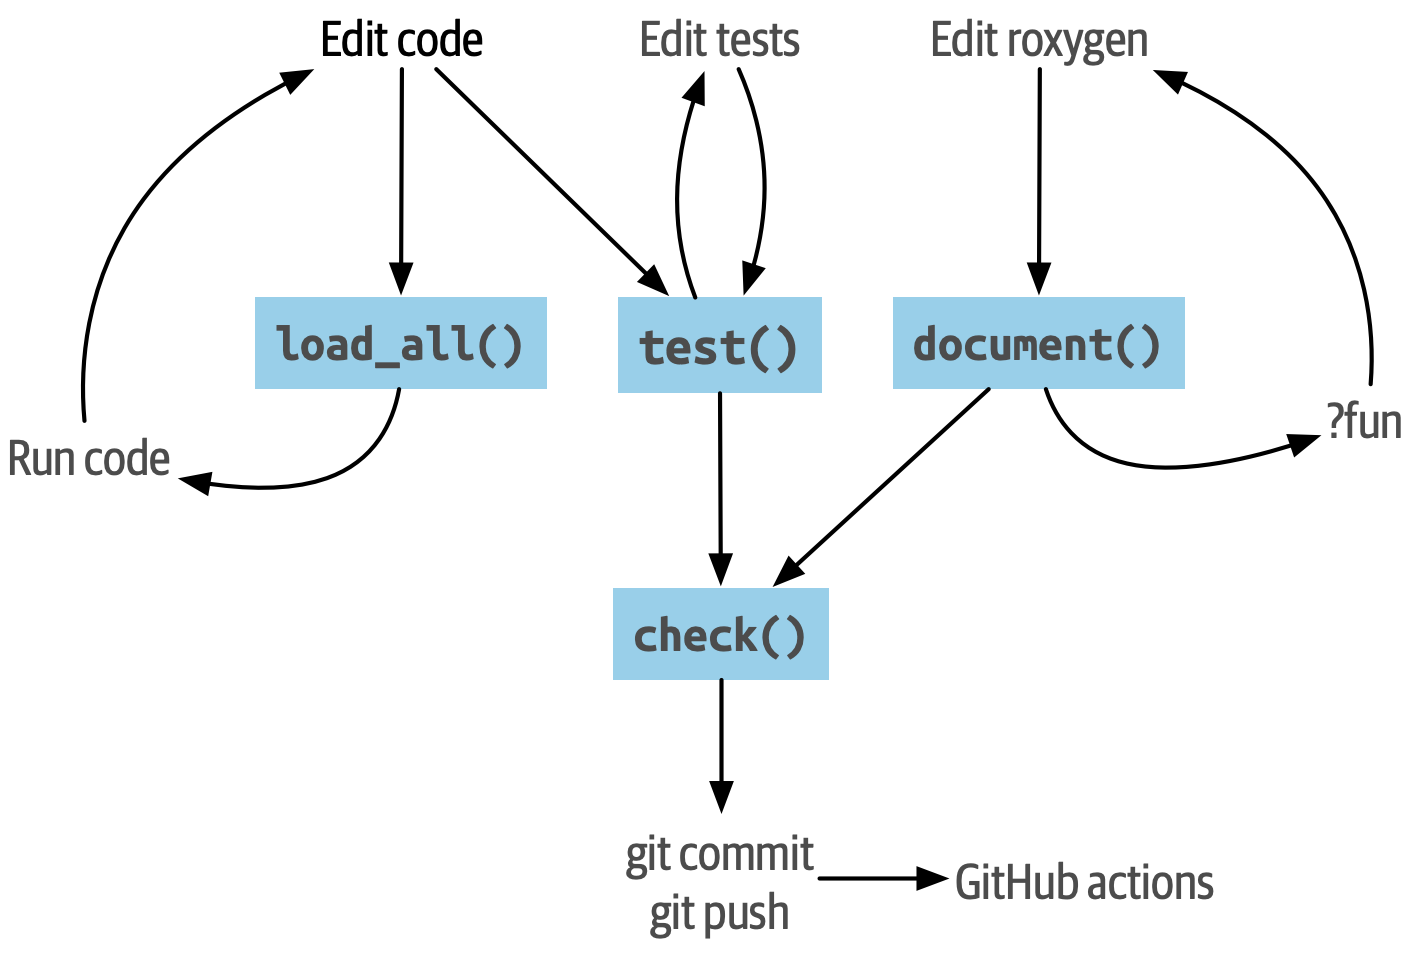
\includegraphics[width=19.61in]{images/package_workflow}

\hypertarget{package-structure}{%
\section{Package Structure}\label{package-structure}}

In an R package or R project structured as a package the typical files and folders will be (locally, you can consult your Files pane):

\begin{tabular}{l|l|l}
\hline
path & type & description\\
\hline
.Rbuildignore & file & Lists files that we need to have around but that should not be included when building the R package from source.\\
\hline
.gitignore & file & Tells Git to ignore some standard, behind-the-scenes files created by R and RStudio.\\
\hline
DESCRIPTION & file & Provides metadata about your package.\\
\hline
NAMESPACE & file & Declares the functions your package exports for external use and the external functions your package imports from other packages.\\
\hline
R/ & folder & the “business end” of your package. It will soon contain .R files with function definitions.\\
\hline
\end{tabular}

\hypertarget{loading-devtools-and-usethis}{%
\section{Loading devtools and usethis}\label{loading-devtools-and-usethis}}

The \texttt{devtools} package is fundamental for developing packages, it comes with a suite of incredibly powerful functions. In addition,
it comes with the required package \texttt{usethis}, which compliments the \texttt{devtools} package with another suite of functions required to properly build packages.

\begin{Shaded}
\begin{Highlighting}[]
\KeywordTok{library}\NormalTok{(devtools)}
\end{Highlighting}
\end{Shaded}

\hypertarget{load}{%
\section{\texorpdfstring{\texttt{load\_all} function}{load\_all function}}\label{load}}

In a package or project structured as a package you are typically making functions that are stored in the \texttt{R/} folder. In a standard project you may be familiar with the use of \texttt{source("R/myfunction.R")} to load or run a script. However, devtools allows us to easily run/load all of our project contents with one simple function call:

\begin{Shaded}
\begin{Highlighting}[]
\NormalTok{devtools}\OperatorTok{::}\KeywordTok{load_all}\NormalTok{()}
\end{Highlighting}
\end{Shaded}

This does a few main things:

\begin{itemize}
\tightlist
\item
  Loads/runs your scripts located in the \texttt{R/} folder\\
\item
  Loads data stored in your \texttt{data} folder\\
\item
  Loads other package objects\\
\item
  Loads package dependencies listed in the \texttt{DESCRIPTION} file
\end{itemize}

\textbf{NOTE}

One main difference is that these functions and data that have been loaded will not appear in the environment, even though they are available. This is similar to when we load a package, such as \texttt{library(tidyverse)}, we are now able to use functions such as \texttt{mutate} even though they don't appear in our environment.

\hypertarget{desc}{%
\section{\texorpdfstring{The \texttt{DESCRIPTION} file}{The DESCRIPTION file}}\label{desc}}

The \texttt{DESCRIPTION} file provides metadata for your package. Some key pieces of this metadata include the description of the project and the dependencies.

If your project doesn't have a \texttt{DESCRIPTION} file you can easily add one using usethis:

\begin{Shaded}
\begin{Highlighting}[]
\NormalTok{usethis}\OperatorTok{::}\KeywordTok{use_description}\NormalTok{()}
\end{Highlighting}
\end{Shaded}

You can manually edit this file or alternatively add certain elements using usethis. For example adding dependencies:

\begin{Shaded}
\begin{Highlighting}[]
\NormalTok{usethis}\OperatorTok{::}\KeywordTok{use_package}\NormalTok{(}\StringTok{'dplyr'}\NormalTok{)}
\end{Highlighting}
\end{Shaded}

\textbf{NOTE}

After creating a \texttt{DESCRIPTION} file in your project you will automatically enter package development mode.

\href{https://r-pkgs.org/description.html}{Read more!}

\hypertarget{documenting-your-functions}{%
\section{Documenting your functions}\label{documenting-your-functions}}

At some point we have all used the help functions in R by easily calling something like \texttt{?mutate}. This requires special documentation which is stored in path such as \texttt{man/mutate} within the package. To do this for ourselves we have to use something called roxygen2, which helps create these handy help windows. To do this with your functions you can open your function script, place the cursor somewhere within the function and then do \emph{Code \textgreater{} Insert roxygen skeleton}, which will create a basic skeleton to fill out such as this:

\begin{Shaded}
\begin{Highlighting}[]
\CommentTok{#' Split a string}
\CommentTok{#'}
\CommentTok{#' @param x A character vector with one element.}
\CommentTok{#' @param split What to split on.}
\CommentTok{#'}
\CommentTok{#' @return A character vector.}
\CommentTok{#' @export}
\CommentTok{#'}
\CommentTok{#' @examples}
\CommentTok{#' x <- "alfa,bravo,charlie,delta"}
\CommentTok{#' strsplit1(x, split = ",")}
\NormalTok{strsplit1 <-}\StringTok{ }\ControlFlowTok{function}\NormalTok{(x, split) \{}
  \KeywordTok{strsplit}\NormalTok{(x, }\DataTypeTok{split =}\NormalTok{ split)[[}\DecValTok{1}\NormalTok{]]}
\NormalTok{\}}
\end{Highlighting}
\end{Shaded}

Now, one more step is needed. We must use devtools to automatically create that \texttt{man/function} and update our \texttt{NAMESPACE} file like so:

\begin{Shaded}
\begin{Highlighting}[]
\NormalTok{devtools}\OperatorTok{::}\KeywordTok{document}\NormalTok{()}
\end{Highlighting}
\end{Shaded}

\href{https://r-pkgs.org/man.html}{Read more!}

\hypertarget{the-namespace}{%
\section{\texorpdfstring{The \texttt{NAMESPACE}}{The NAMESPACE}}\label{the-namespace}}

The \texttt{NAMESPACE} file is an automatically generated and maintaind file by R, this should not be manually modified. It is filled out depending on the roxygen2 comments left in your scripts and is updated, as described above, by using \texttt{devtools::document()}. It informs the package what contents should be exported when building the package, as well as what needs to be imported (package dependencies) for the package to run.

\href{https://r-pkgs.org/dependencies-mindset-background.html\#sec-dependencies-namespace}{Read more!}

\hypertarget{the-readme-file}{%
\section{\texorpdfstring{The \texttt{README} file}{The README file}}\label{the-readme-file}}

The \texttt{README} file is a very useful document that can help provide context, general information, and usage insight to users. In addition, when knitted, \texttt{README} files are formatted to appear as nice markdown documents in Github and Gitlab.

To get a \texttt{README} file started in a project all that you need to do is:

\begin{Shaded}
\begin{Highlighting}[]
\NormalTok{usethis}\OperatorTok{::}\KeywordTok{use_readme_rmd}\NormalTok{() }
\end{Highlighting}
\end{Shaded}

\textbf{NOTE}

Remember, you have to knit your \texttt{README} in order to produce a \texttt{.md} file version of it, which will be directly used in places like Github or Gitlab.

\hypertarget{organizing-your-scripts}{%
\section{Organizing your scripts}\label{organizing-your-scripts}}

The file name should be meaningful and convey which functions are defined within. While you're free to arrange functions into files as you wish, the two extremes are bad: don't put all functions into one file and don't put each function into its own separate file.

\begin{tabular}{l|l}
\hline
Organizing.principle & Comments\\
\hline
One function & Defines exactly one function, that’s not particulary large, but doesn’t fit naturally into any other .R file\\
\hline
Main function plus helpers & Defines the user-facing function, a method, and private helpers\\
\hline
Family of functions & Defines a family of functions, all documented together in a big help topic, plus private helpers\\
\hline
\end{tabular}

\textbf{TIP}

Another file you often see in the wild is \texttt{R/utils.R}.
This is a common place to define small utilities that are used inside multiple package functions.
Since they serve as helpers to multiple functions, placing them in \texttt{R/utils.R} makes them easier to re-discover when you return to your package after a long break.

\hypertarget{pkg-data}{%
\section{Using data in a package}\label{pkg-data}}

Traditionally, data in a package is stored in the \texttt{data/} folder. The data there will be saved in a specific data form that will make it available when you run \texttt{devtools::load\_all()}. To store data within a package like this you need to run:

\begin{Shaded}
\begin{Highlighting}[]
\NormalTok{usethis}\OperatorTok{::}\KeywordTok{use_data}\NormalTok{(df)}
\end{Highlighting}
\end{Shaded}

\hypertarget{additional-resources-1}{%
\section{Additional Resources}\label{additional-resources-1}}

\begin{itemize}
\tightlist
\item
  \href{https://r-pkgs.org/}{R Package Manual}
\end{itemize}

\hypertarget{shiny}{%
\chapter{Shiny}\label{shiny}}

If you've never used Shiny before, welcome! Shiny is an R package that allows you to easily create rich, interactive web apps. Shiny allows you to take your work in R and expose it via a web browser so that anyone can use it. Shiny makes you look awesome by making it easy to produce polished web apps with a minimum amount of pain.

\hypertarget{shiny-app-structure}{%
\section{Shiny App Structure}\label{shiny-app-structure}}

Shiny apps are composed of two main elements.

\begin{itemize}
\tightlist
\item
  The UI: This is where you define the layout and appearance of your app, including sliders, plots, tabs, etc.
\item
  The server: This is where you connect your UI components using logic behind the scenes to drive app behaviour.
\end{itemize}

These two elements are operationalized by calling \texttt{shinyApp(ui\ =\ ui,\ server\ =\ server)}

\hypertarget{ui}{%
\section{UI}\label{ui}}

\hypertarget{setting-up-the-ui}{%
\subsection{Setting up the UI}\label{setting-up-the-ui}}

TO create a shiny app you must create a UI. Traditionally, using shiny you would do this using the function \texttt{fluidPage()}. The UI will contain elements such as calls to CSS stylings, overall UI design, inputs, and outputs.

\hypertarget{layout-and-themes}{%
\subsection{Layout and themes}\label{layout-and-themes}}

al lof the page layouts and panels, sidebars

CSS

html

\hypertarget{inputs}{%
\subsection{Inputs}\label{inputs}}

There are a number of inputs that are incredibly useful in shiny apps such as \texttt{radioButtons()}, \texttt{selectInput()}, \texttt{actionButton()}, and \texttt{dateRangeInput()}. These allow users to interact with our app to dictate what appears in our app.

These functions all share a two main arguments:

\begin{itemize}
\tightlist
\item
  \texttt{inputID}: This is the identifier used to connect the front end with the back end: if your UI has an input with ID ``name'', the server function will access it with input\$name.\\
\item
  \texttt{label}: This is used to create a human-readable label for the control (ie. Select Geography).
\end{itemize}

\textbf{NOTE}

The \texttt{inputId} has two constraints:

\begin{itemize}
\item
  It must be a simple string that contains only letters, numbers, and underscores (no spaces, dashes, periods, or other special characters allowed!). Name it like you would name a variable in R.
\item
  It must be unique. If it's not unique, you'll have no way to refer to this control in your server function!
\end{itemize}

\hypertarget{outputs}{%
\subsection{Outputs}\label{outputs}}

In the UI we can also specify the outputs that we'd like to include, for example plots, text, or tables. In essence, these are `placeholders', which will be filled in based on what we define in our server. Similar to inputs, we must also specify an \texttt{inputID} as the first argument.

\hypertarget{server}{%
\section{Server}\label{server}}

On the server side, we need to use a different suite of functions that will focus on three main things:

\begin{itemize}
\tightlist
\item
  Inputs: these are referenced by calling their IDs using \texttt{input\$button1} for example.
\item
  Outputs: Because we set up our `placeholders' in the UI we need to tell them what to be filled with here (ie. render a plot).
\item
  Reactivity: these will determine the behaviour of your app, typically in response to things like \texttt{input\$button1}.
\end{itemize}

\hypertarget{dynamic-ui}{%
\section{Dynamic UI}\label{dynamic-ui}}

\hypertarget{basic-example}{%
\section{Basic example}\label{basic-example}}

\hypertarget{deploying-your-app}{%
\section{Deploying your app}\label{deploying-your-app}}

\hypertarget{packaging-a-shiny-app}{%
\section{Packaging a Shiny App}\label{packaging-a-shiny-app}}

Using package structure for a shiny app gets your toes into the water of package development. It's a long way from a complete package, but it's still useful because it activates new tools that make it easier to work with larger app and provides you with standard conventions that can be used across projects.

\hypertarget{put-all-r-code-in-the-r-directory}{%
\subsection{\texorpdfstring{Put all R code in the \texttt{R/} directory}{Put all R code in the R/ directory}}\label{put-all-r-code-in-the-r-directory}}

Because we are going to be working in an app-package we need to create an \texttt{R/} directory. This is where we will keep all of the core R code components that will build our app. As a reminder, in a package we are leveraging useful tools like \texttt{devtools::load\_all()} (See section \ref{load}), which will go into the \texttt{R/} directory and load/run all of the code within this directory.

\hypertarget{write-a-function-that-starts-your-app}{%
\subsection{Write a function that starts your app}\label{write-a-function-that-starts-your-app}}

As mentioned in section (LINK HERE), we need three primary pieces to create an app:

\begin{Shaded}
\begin{Highlighting}[]
\NormalTok{ui <-}\StringTok{ }\KeywordTok{fluidPage}\NormalTok{(}
\NormalTok{  ...}
\NormalTok{)}

\NormalTok{server <-}\StringTok{ }\ControlFlowTok{function}\NormalTok{(input, output, session) \{}
\NormalTok{  ...}
\NormalTok{\}}

\KeywordTok{shinyApp}\NormalTok{(ui, server, ...)}
\end{Highlighting}
\end{Shaded}

Now, to begin converting our project to a package-app we must wrap this into a function:

\begin{Shaded}
\begin{Highlighting}[]
\NormalTok{myApp <-}\StringTok{ }\ControlFlowTok{function}\NormalTok{(...) \{}
\NormalTok{  ui <-}\StringTok{ }\KeywordTok{fluidPage}\NormalTok{(}
\NormalTok{    ...}
\NormalTok{  )}
\NormalTok{  server <-}\StringTok{ }\ControlFlowTok{function}\NormalTok{(input, output, session) \{}
\NormalTok{    ...}
\NormalTok{  \}}
  \KeywordTok{shinyApp}\NormalTok{(ui, server, ...)}
\NormalTok{\}}
\end{Highlighting}
\end{Shaded}

\textbf{NOTE}

The function you create shouldn't need any arguments, all that we will use this for is to easily run our app locally and set it up for easy deployment later.

\hypertarget{save-your-data-to-the-data-directory}{%
\subsection{\texorpdfstring{Save your data to the \texttt{data/} directory}{Save your data to the data/ directory}}\label{save-your-data-to-the-data-directory}}

We may have some datasets or lists that we use in our app that aren't routinely updated. These are perfect candidates to convert into \texttt{.rda} files using the handy function \texttt{usethis::use\_data()} that we talked about in section \ref{pkg-data}. These will automatically be stored in the \texttt{data/} directory and can be easily called directly after running \texttt{load\_all()}.

\hypertarget{create-an-inst-directory}{%
\subsection{\texorpdfstring{Create an \texttt{inst/} directory}{Create an inst/ directory}}\label{create-an-inst-directory}}

The \texttt{inst/} directory is where we can store other raw datasets that are more subject to change, for example the data used to feed our apps that comes from external pipelines. There is no standard convention so you can name things as you please, but common usage includes folders named \texttt{inst/extdata} or \texttt{inst/ext} to store these datasets.

\textbf{NOTE}

Load data with \texttt{read.csv(system.file("exdata",\ "mydata.csv",\ package\ =\ "myApp"))}. Notice that our package-app automatically knows to look in our \texttt{inst/} folder?

\begin{Shaded}
\begin{Highlighting}[]
\NormalTok{myApp <-}\StringTok{ }\ControlFlowTok{function}\NormalTok{(...) \{}
  \KeywordTok{read.csv}\NormalTok{(}\KeywordTok{system.file}\NormalTok{(}\StringTok{"extdata"}\NormalTok{, }\StringTok{"mydata.csv"}\NormalTok{, }\DataTypeTok{package =} \StringTok{"myApp"}\NormalTok{))}
\NormalTok{  ui <-}\StringTok{ }\KeywordTok{fluidPage}\NormalTok{(}
\NormalTok{    ...}
\NormalTok{  )}
\NormalTok{  server <-}\StringTok{ }\ControlFlowTok{function}\NormalTok{(input, output, session) \{}
\NormalTok{    ...}
\NormalTok{  \}}
  \KeywordTok{shinyApp}\NormalTok{(ui, server, ...)}
\NormalTok{\}}
\end{Highlighting}
\end{Shaded}

\hypertarget{create-a-www-directory}{%
\subsection{\texorpdfstring{Create a \texttt{www/} directory}{Create a www/ directory}}\label{create-a-www-directory}}

This directory is where you can store some of the other non-script or data components to the app such as CSS stylings or images. There are no rules to this but a suggestion would be to have a \texttt{www/css} and \texttt{www/images} sub-directory scheme for your app.

\textbf{TIP}

If you want to call files from within these sub-directories (eg. \texttt{href\ =\ "css/style.css"}) you will need to tell your app where they are:

\begin{Shaded}
\begin{Highlighting}[]
\NormalTok{myApp <-}\StringTok{ }\ControlFlowTok{function}\NormalTok{(...) \{}
\NormalTok{  shiny}\OperatorTok{::}\KeywordTok{addResourcePath}\NormalTok{(}\StringTok{"css"}\NormalTok{, }\KeywordTok{file.path}\NormalTok{(}\KeywordTok{getwd}\NormalTok{(), }\StringTok{"www/css"}\NormalTok{))}
\NormalTok{  shiny}\OperatorTok{::}\KeywordTok{addResourcePath}\NormalTok{(}\StringTok{"images"}\NormalTok{, }\KeywordTok{file.path}\NormalTok{(}\KeywordTok{getwd}\NormalTok{(), }\StringTok{"www/images"}\NormalTok{))}
\NormalTok{  ui <-}\StringTok{ }\KeywordTok{fluidPage}\NormalTok{(}
\NormalTok{    ...}
\NormalTok{  )}
\NormalTok{  server <-}\StringTok{ }\ControlFlowTok{function}\NormalTok{(input, output, session) \{}
\NormalTok{    ...}
\NormalTok{  \}}
  \KeywordTok{shinyApp}\NormalTok{(ui, server, ...)}
\NormalTok{\}}
\end{Highlighting}
\end{Shaded}

\hypertarget{create-a-description-file}{%
\subsection{\texorpdfstring{Create a \texttt{DESCRIPTION} file}{Create a DESCRIPTION file}}\label{create-a-description-file}}

Because we are working in a package environment one of the critical components will be our \texttt{DESCRIPTION} file, which was discussed in section \ref{desc}. Don't forget to set your dependencies!

\hypertarget{deploying-your-app-package}{%
\subsection{Deploying your app-package}\label{deploying-your-app-package}}

One of the final pieces to setting up your app-package is the \texttt{app.R} script. This is what will be used when we go to deploy our app to the server and contains two simple but important lines of code:

\begin{Shaded}
\begin{Highlighting}[]
\NormalTok{pkgload}\OperatorTok{::}\KeywordTok{load_all}\NormalTok{(}\StringTok{"."}\NormalTok{)}
\KeywordTok{myApp}\NormalTok{()}
\end{Highlighting}
\end{Shaded}

\textbf{WARNING}

Although this is an R script, we \textbf{DO NOT} place this under our \texttt{R/} directory. This would result in an infinite loop when loading due to our \texttt{load\_all()} function! Therefore place this at the top-level of your project directory.

Normally when you deploy an app, the rsconnect package automatically figures out all of the packages your code uses. But now that you have a \texttt{DESCRIPTION} file, it requires you to explicitly specify them. The easiest way to do this is to call usethis::use\_package(). You'll need to start with shiny and pkgload:

\begin{Shaded}
\begin{Highlighting}[]
\NormalTok{usethis}\OperatorTok{::}\KeywordTok{use_package}\NormalTok{(}\StringTok{"shiny"}\NormalTok{)}
\NormalTok{usethis}\OperatorTok{::}\KeywordTok{use_package}\NormalTok{(}\StringTok{"pkgload"}\NormalTok{)}
\end{Highlighting}
\end{Shaded}

\href{https://mastering-shiny.org/scaling-packaging.html\#deploying-your-app-package}{Read more!}

\hypertarget{workflow}{%
\subsection{Workflow}\label{workflow}}

Putting your app code into the package structure unlocks a new workflow:

\begin{itemize}
\item
  Re-load all code in the app with \texttt{Cmd/Ctrl\ +\ Shift\ +\ L}. This calls \texttt{devtools::load\_all()} which automatically saves all open files, \texttt{source()}s every file in \texttt{R/}, loads all datasets in \texttt{data/} then puts your cursor in the console.
\item
  Re-run the app with \texttt{myApp()}.
\end{itemize}

\href{https://mastering-shiny.org/scaling-packaging.html\#workflow}{Read more!}

\hypertarget{additional-resources-2}{%
\section{Additional Resources}\label{additional-resources-2}}

\begin{itemize}
\tightlist
\item
  \href{https://mastering-shiny.org/}{Shiny Manual}\\
\item
  \href{https://rstudio.github.io/cheatsheets/html/shiny.html}{Shiny Cheatsheet}
\end{itemize}

\hypertarget{bslib}{%
\chapter{bslib}\label{bslib}}

\hypertarget{section}{%
\section{}\label{section}}

.

\hypertarget{modularization}{%
\chapter{Modularization}\label{modularization}}

\hypertarget{section-1}{%
\section{}\label{section-1}}

.

  \bibliography{book.bib,packages.bib}

\end{document}
